% Chapter 10

\chapter{Systematic Uncertainties} % Chapter title

\label{ch:backgrounds} 

\section{Uncertainties on Data-Driven Backgrounds}

\subsection{Uncertainties on the Flavor Symmetry Method}
\label{sec:unc_fs}

The flavor symmetry method is a data driven method that makes its primarily on based events populating an \ac{SR}-like \ac{CR} in the different-flavor channel. The statistical uncertainty on these events makes up the dominant uncertainty on the method. To reduce this uncertainty, the \mll range on the \ac{CR} is expanded, tripling the number of events in CR-FS. Though this reduces the statistical uncertainty significantly, it is still significantly higher than any of the other systematic uncertainties on this method, as seen in \autoref{tab:fs_errors}. Also included in the statistical uncertainty column is the uncertainty on the number of non-\ac{FS} events in CR-FS, which is used to scale the prediction to remove any contamination in the \ac{CR}. 

\begin{table}[!ht]
\begin{center}
 \begin{tabular}{lcc|cccccc}
 \hline 
 \multirow{3}{*}{Reg.}	& \multirow{3}{*}{Ch.} 	& \multirow{3}{*}{Pred.} & \multicolumn{6}{c}{Uncertainties} \\
   \cline{4-9} 
   		 	& 		 	& 	  		& stat.  		& MC 		& k  			& dAOD 		& \mll  	& total \\
   			& 			& 		 	& 			 	& clos. 	& and $\alpha$	& usage	 	& shape  	& \\
   \hline
   \hline
\multirow{3}{*}{SRZ}
& $ee$ & 16.50 & 1.82 & 0.88 & 0.53 & 0.12 & 0.22 & 2.11 \\ 
& $\mu\mu$ & 16.67 & 1.83 & 0.79 & 0.33 & 0.11 & 0.23 & 2.04 \\ 
& $ee$+$\mu\mu$ & 33.16 & 3.66 & 1.07 & 0.86 & 0.23 & 0.45 & 3.94 \\ 
\hline
\multirow{3}{*}{VRS}
& $ee$ & 49.70 & 3.21 & 2.34 & 2.20 & 0.34 & 0.75 & 4.61 \\ 
& $\mu\mu$ & 49.60 & 3.14 & 2.88 & 1.40 & 0.31 & 0.75 & 4.56 \\ 
& $ee$+$\mu\mu$ & 99.31 & 6.34 & 4.00 & 3.60 & 0.65 & 1.49 & 8.47 \\ 
\hline
 
\hline
\hline
 \end{tabular}
\end{center}
 \caption{
   Uncertainties in the on-Z signal and validation regions. Nominal predictions are given with statistical uncertainty (including uncertainty from subtracted backgrounds), MC Closure uncertainty, uncertainty on the prediction from varying k and $\alpha$ by their statistical uncertainties, comparing the efficiencies from AODs to that of DAODs, and on the \mll widening, which includes MC statistics and a data/MC comparison in a loosened region.
 }
 \label{tab:fs_errors}
\end{table}

The next largest contribution to the uncertainty comes from \ac{MC} closure tests, which are used to determine how effective the method is in its prediction. If, for example, using weights derived from an inclusive selection at high \met lead to a bias, the closure test would indicate that and an appropriate uncertainty could be placed on the estimate based on the difference between the \ac{MC} and the prediction. In this test, the entire \ac{FS} procedure is performed on \ttbar \ac{MC}, including a recalculation of weighting factors $\alpha$ and $k$. The prediction from $e\mu$ events in \ac{MC} is compared to the \ac{MC} $ee$ and $\mu\mu$ events, as seen in \autoref{fig:fs_closure}. The difference between the two predictions is then summed in quadrature with the statistical uncertainty on each prediction to give the total closure uncertainty seen in \autoref{tab:fs_errors}. In these closure tests, all predictions agree within the statistical uncertainty, so the bulk of the resulting error is due to \ac{MC} statistics. 

\begin{centering}
\begin{figure}[!ht]
\myfloatalign
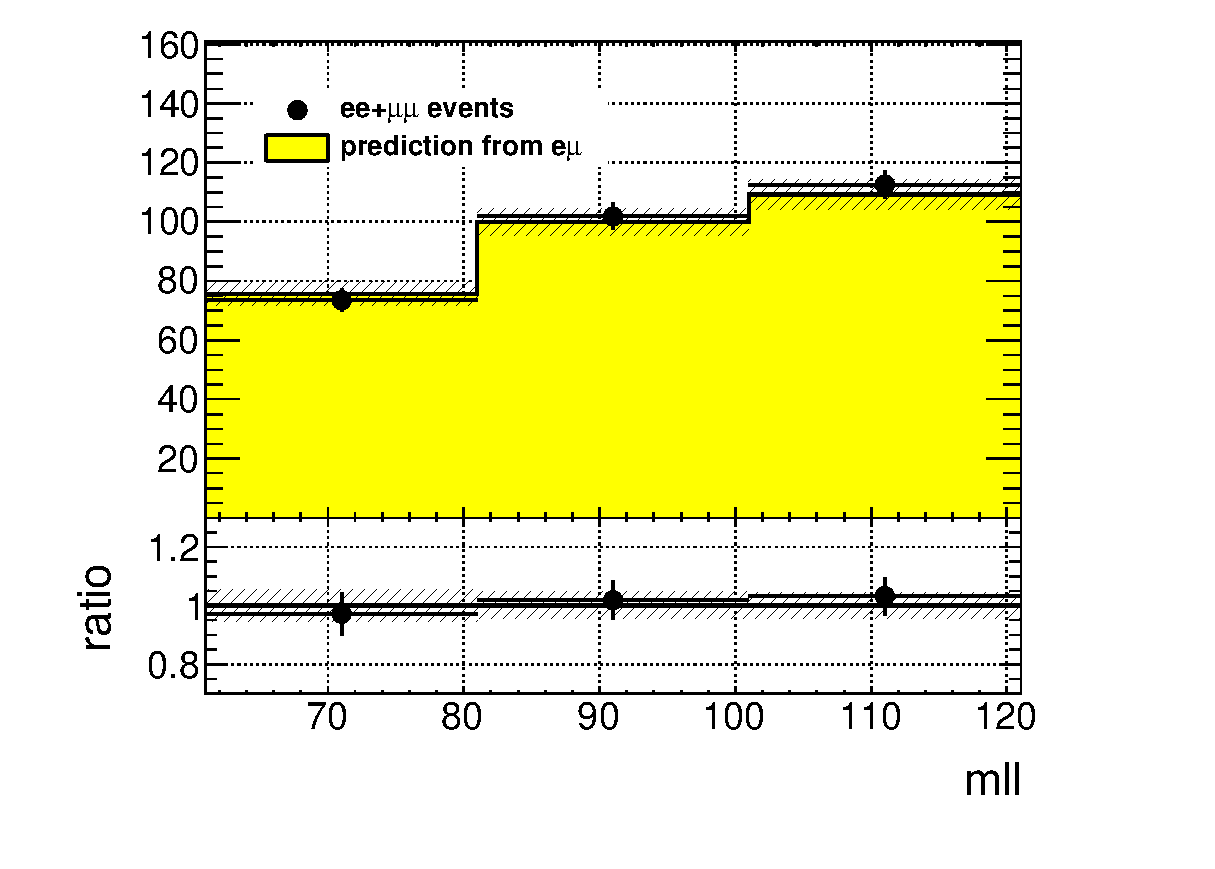
\includegraphics[width=.85\linewidth]{figures/fs/ee+mm_ratio_mll_VRZ_widened.eps}
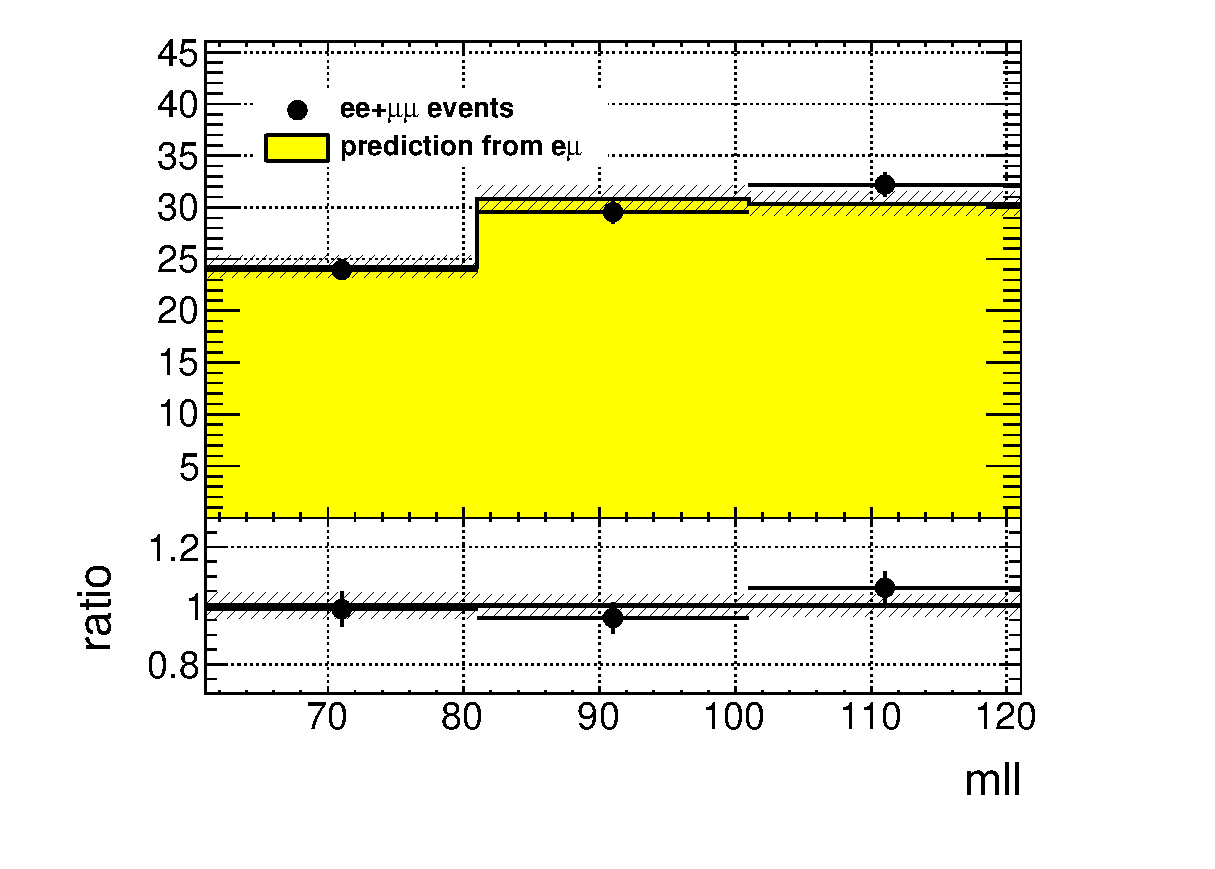
\includegraphics[width=.85\linewidth]{figures/fs/ee+mm_ratio_mll_SRZ_widened.eps}
\caption{MC closure plots of VRS (top) and SRZ (bottom). The number of events from MC (black points) is compared to the number of events predicted from the flavor symmetry method (yellow histogram). The comparison is performed before the expanded \mll window is used to predict the on-$Z$ bin.}
\label{fig:fs_closure}
\end{figure}
\end{centering}

A small uncertainty is added based on the statistical uncertainty on the $k$ and $\alpha$ factors derived from data. These factors are measured in many different bins (see, for example, the different measurements of $k$ in \autoref{fig:fs_k}), and as a consequence, some bins can have very large statistical uncertainties. To assess the uncertainty on the total estimate, each measurement of these factors is varied by its uncertainty in order to produce the maximum and minimum possible prediction. This error is symmetrized, and the resulting change in the prediction is included in \autoref{tab:fs_errors}.

\begin{centering}
\begin{figure}[bth]
\myfloatalign
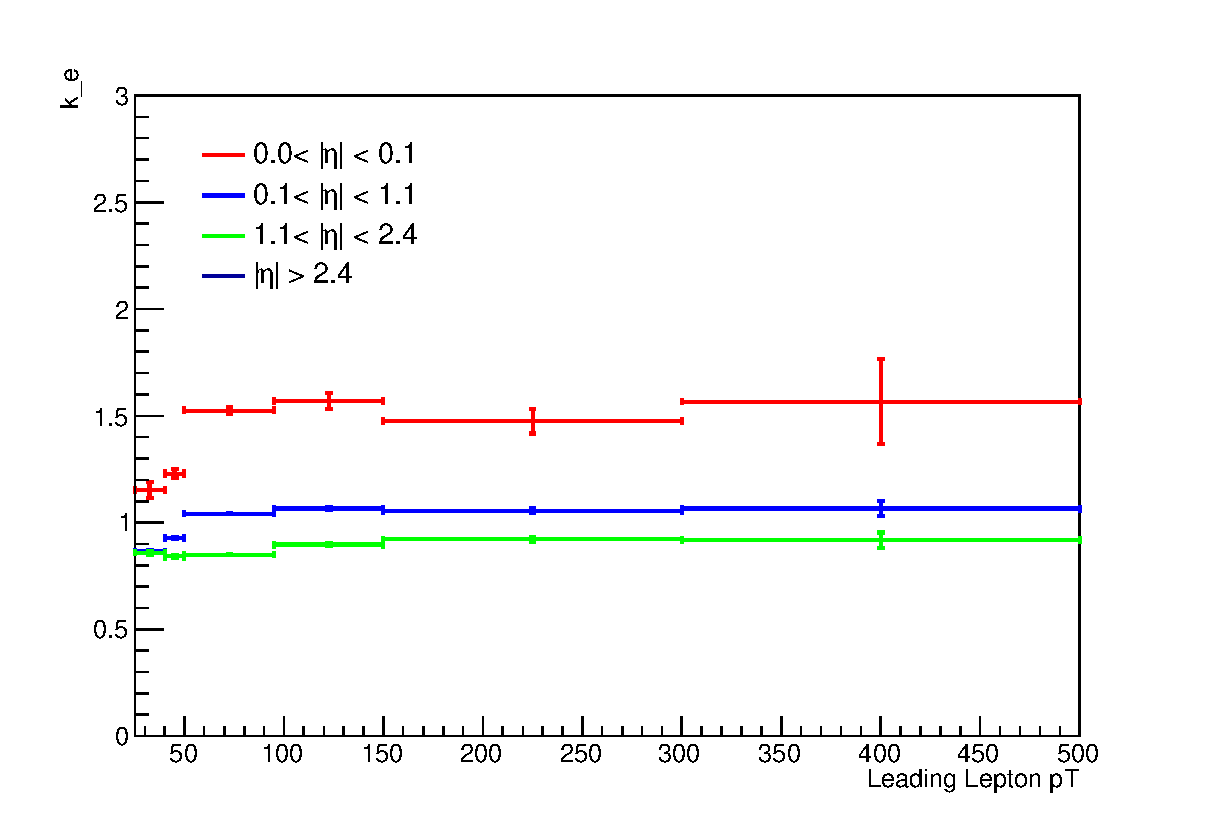
\includegraphics[width=.85\linewidth]{figures/fs/data_efficiencies_2j_Z_lep0.eps}
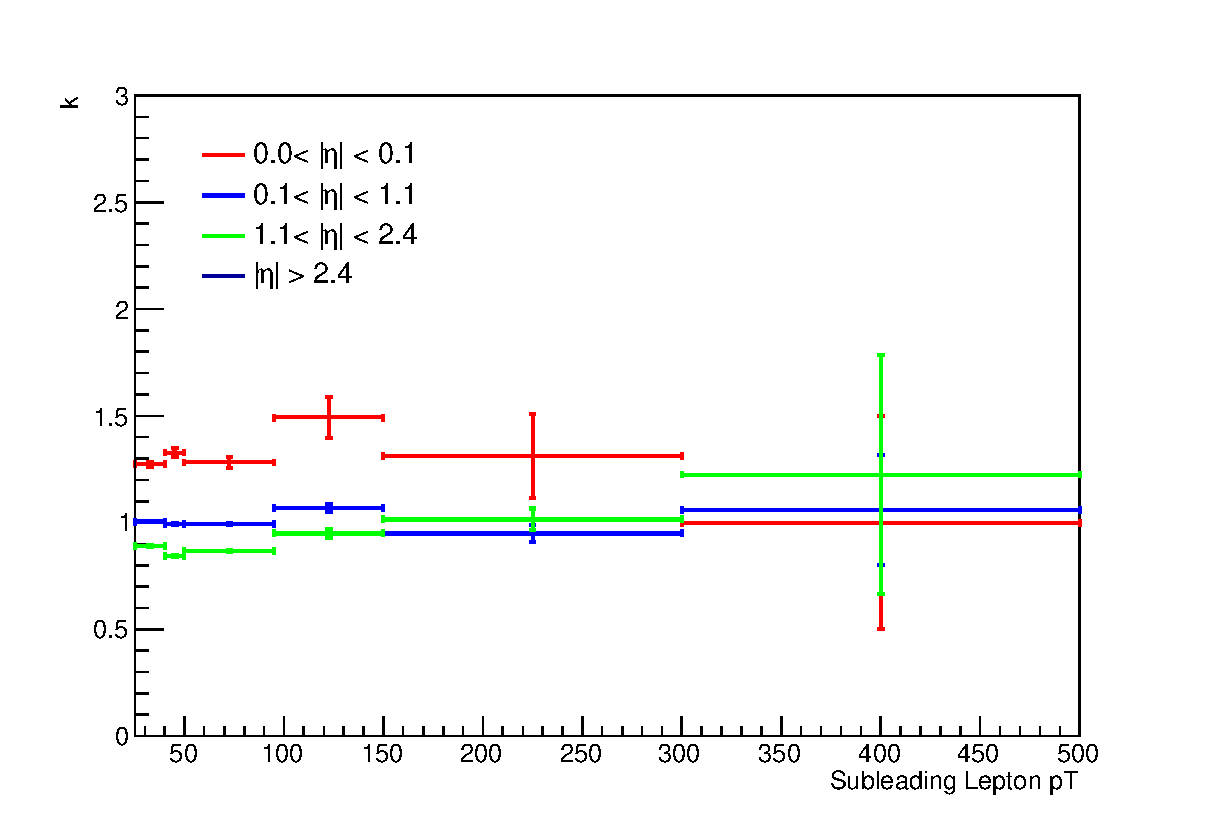
\includegraphics[width=.85\linewidth]{figures/fs/data_efficiencies_2j_Z_lep1.eps}
\caption{Measurements of $k$, the ratio of electron to muon events, in bins of $\pT$ and $\eta$. On the top is the measurements indexed by the leading lepton, while the measurements indexed by the subleading lepton are on the bottom. These efficiencies are for the 2016 dataset.}
\label{fig:fs_k}
\end{figure}
\end{centering}

The next uncertainty considers a potential bias in the way the $\alpha$ factors are calculated. Because they are derived from data, there is already trigger dependence in data collection (only events passing a trigger are stored) and further dependences is introduced by the use of the ``dAOD'' data format. This is short for derived \ac{AOD}, and they provide smaller, more efficient versions of the complete ATLAS datasets. These dAODs are designed with specific analyses in mind, filtering on the triggers and objects required by the analyses. As a consequence, there are explicit requirements that lepton or \met triggers are passed before events are included in the dAODs used by this analysis. These requirements mean that the trigger efficiencies calculated from these samples do not include all possible events, and will have artificially high values. However, because the ratio of trigger efficiencies is the quantity needed for this analysis (see \autoref{eq:kandalpha}), this will only bias the prediction if the different channels are differently impacted by the trigger preselection.

Calculating the \ac{FS} prediction's dependence on these biases requires the use of \ac{MC}. With a generated \ac{MC} sample, there is no trigger dependence, so an unskimmed sample can be compared to a typical \ac{MC} dAOD to identify the effect of the skimming. \autoref{fig:fs_alpha} shows a comparison of the $\alpha$ factors calculated for different bins in \met from the nominal source, data, as well as these two \ac{MC} sources. A \met dependence would be the most likely bias between the two \ac{MC}-derived $\alpha$ factors because \met triggers are the only triggers besides lepton triggers that will allow an event to be accepted into the dAOD used by this analysis. Though there is some difference between the data-derived $\alpha$ and those taken from \ac{MC}, it is clear from this plot that there is very little dependence on the choice of an unskimmed or skimmed sample. The actual calculation of the uncertainty is performed by repeating the flavor symmetric method in \ac{MC} with each of the two $\alpha$ factors and observing the difference between the estimates.

\begin{centering}
\begin{figure}[bth]
\myfloatalign
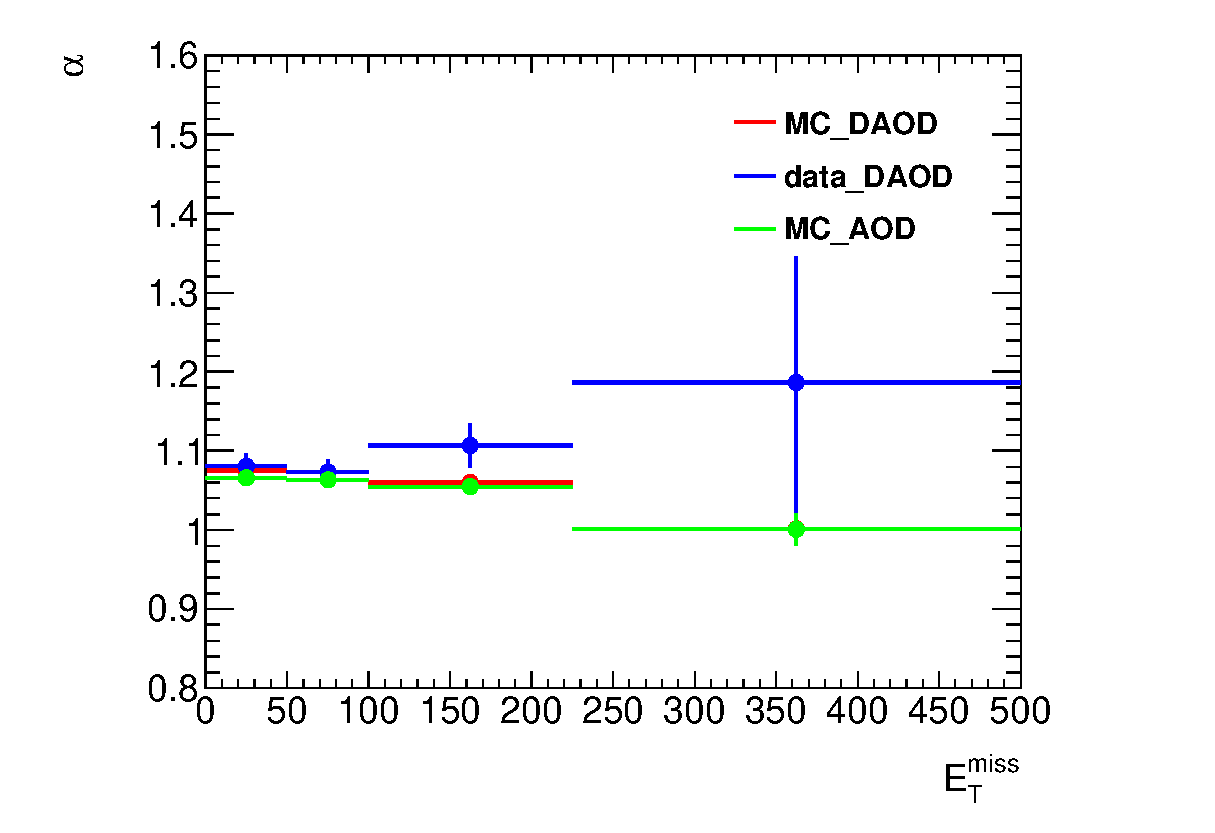
\includegraphics[width=.85\linewidth]{figures/fs/trigger_ratios.eps}
\caption{$\alpha$, the trigger efficiency ratio, calculated as a function of \met from three different sources: data, the usual skimmed \ttbar \ac{MC}, and an unskimmed \ttbar \ac{MC}.}
\label{fig:fs_alpha}
\end{figure}
\end{centering}

The last uncertainty relates to the main \ac{MC} dependence of the method - the \mll shape of the \ac{FS} background. A correction factor is taken from \ac{MC} in order to account for the \mll widening, and the accuracy of that factor must be checked. Its shape is compared to that of data in region similar to VR-FS, but with an \HT cut lowered to 300 \gev to increase statistics. The difference between the fraction of events on the $Z$ mass peak in data and \ac{MC} in this region is taken as a systematic uncertainty. To confirm that using this lowered \HT cut still gives a valid answer, the fractions are compared as a function of \HT in \autoref{fig:fs_frac_ht}. In these plots, especially in the higher-statistics 2016 plot, it is clear both that the data and \ac{MC} agree very well and that there is no strong \HT dependence. 

\begin{centering}
\begin{figure}[bth]
\myfloatalign
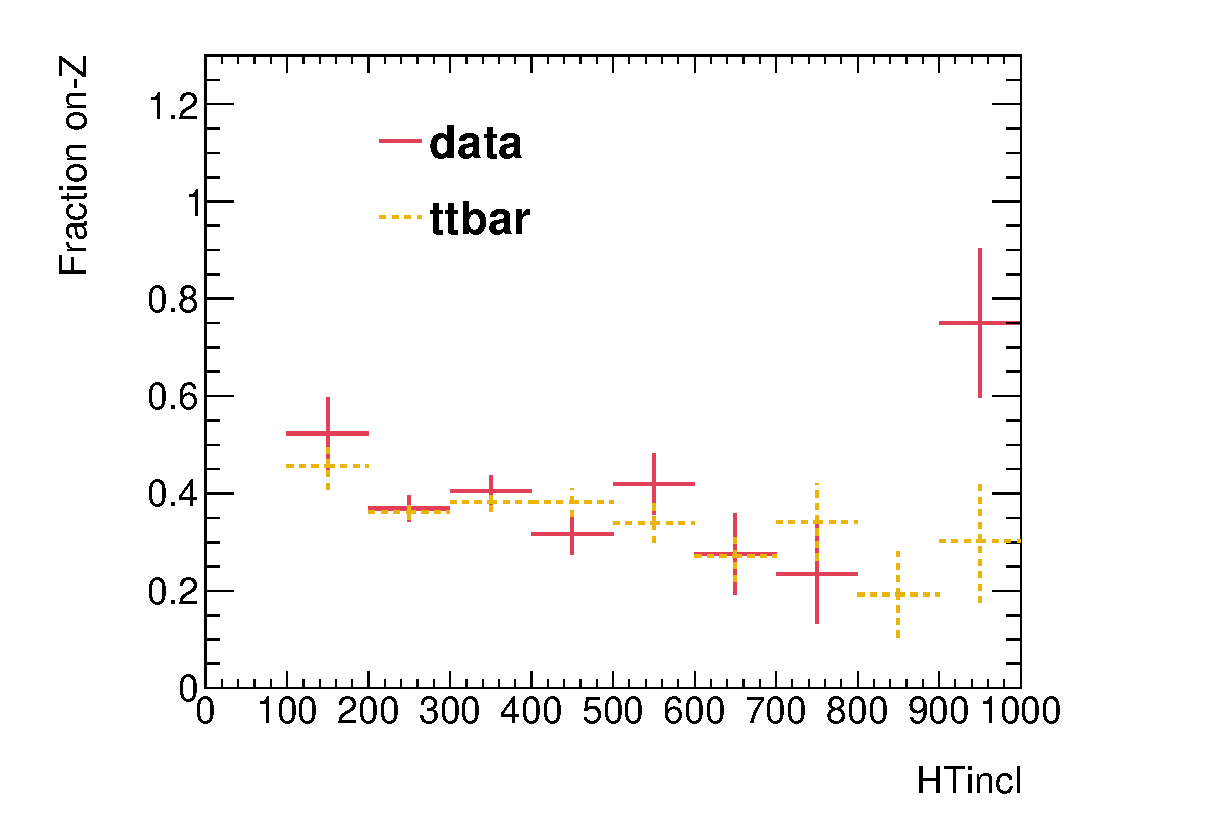
\includegraphics[width=.85\linewidth]{figures/fs/frac_vs_ht_2015.eps}
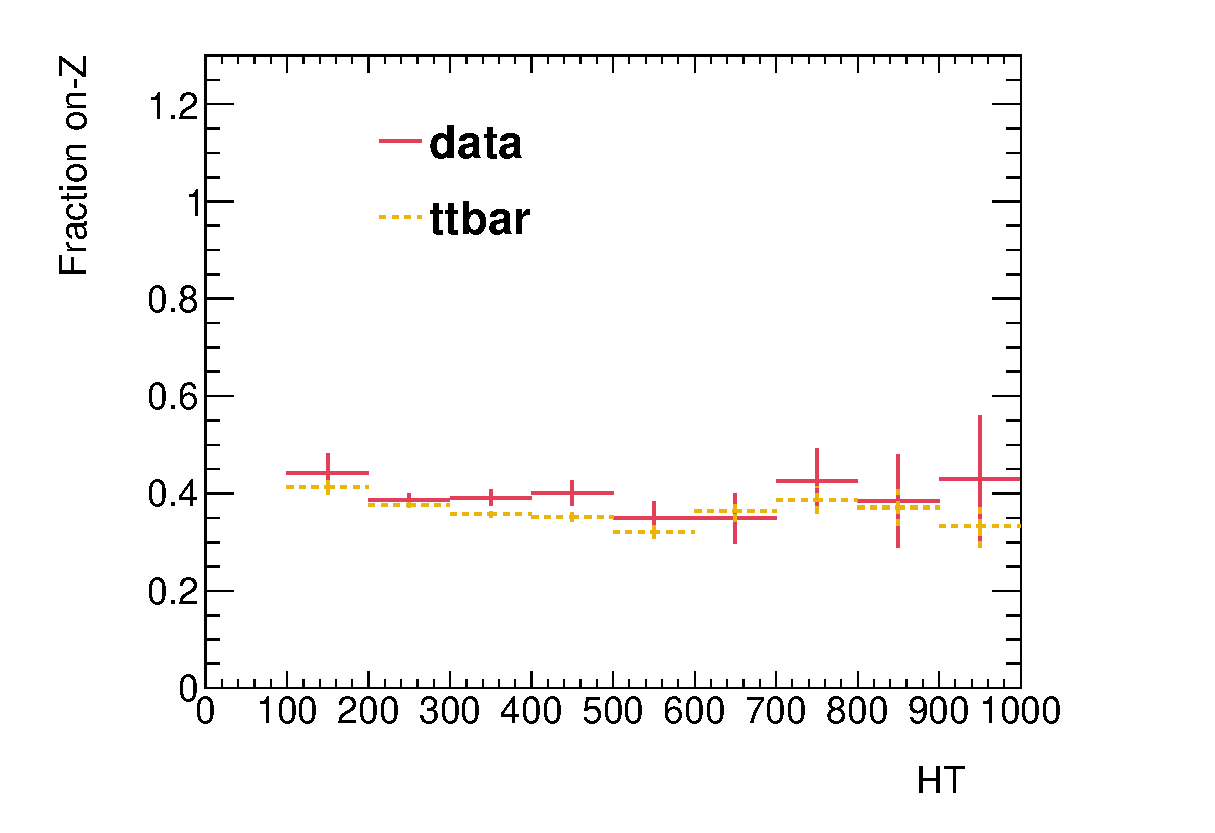
\includegraphics[width=.85\linewidth]{figures/fs/frac_vs_ht_2016.eps}
\caption{Plots of the fraction of on-Z events with a VR-FS-like selection as a function of \HT. The top figure shows 2015 data and \ac{MC} while the bottom figure shows the same for 2016.}
\label{fig:fs_frac_ht}
\end{figure}
\end{centering}

These uncertainties are each calculated independently for the two datasets then added. Statistical uncertainties, including the \ac{MC} closure statistical uncertainties and the $k$ and $\alpha$ uncertainties, are added in quadrature between the two years. Uncertainties that are more likely to be correlated, such as the difference between the two estimates in \ac{MC} closure and the dependence on using a dAOD to calculate trigger efficiencies, are added linearly. The total uncertainty is about 12\% of the nominal prediction in the signal region and about 9\% in the validation region. 

%----------------------------------------------------------------------------------------

\subsection{Uncertainties on the $\gamma$+jets Method}

%----------------------------------------------------------------------------------------

\subsection{Uncertainties on the Fakes Background}

%----------------------------------------------------------------------------------------

\section{Experimental Uncertainties}

%----------------------------------------------------------------------------------------

\section{Theoretical Uncertainties}

%----------------------------------------------------------------------------------------

\section{Signal Uncertainties}

%----------------------------------------------------------------------------------------

\section{Impact of Uncertainties on the Signal Region}

%----------------------------------------------------------------------------------------